\documentclass{article}
\usepackage[a4paper, margin=5em]{geometry}
\usepackage{fancyhdr}
\usepackage{lastpage}
\usepackage{graphicx}
\usepackage{hyperref}
\usepackage{ngerman}
\usepackage{enumitem}
\usepackage{csquotes}
\usepackage{caption}

\newcommand{\gqq}[1]{\glqq{}#1\grqq{}}

\pagestyle{fancy}
\fancyhf{}
\renewcommand{\headrulewidth}{0pt}
\fancyfoot{}

\lfoot{}
\cfoot{Seite \thepage\ / \pageref*{LastPage}}
\rfoot{}

\hypersetup{
    colorlinks=true,
    linktoc=all,
    urlcolor=blue
}

\author{Tim Wende}
\date{\today}
\title{\textbf{Hausaufgabe 5}}

\begin{document}
    \maketitle

    \begin{figure}[ht]
        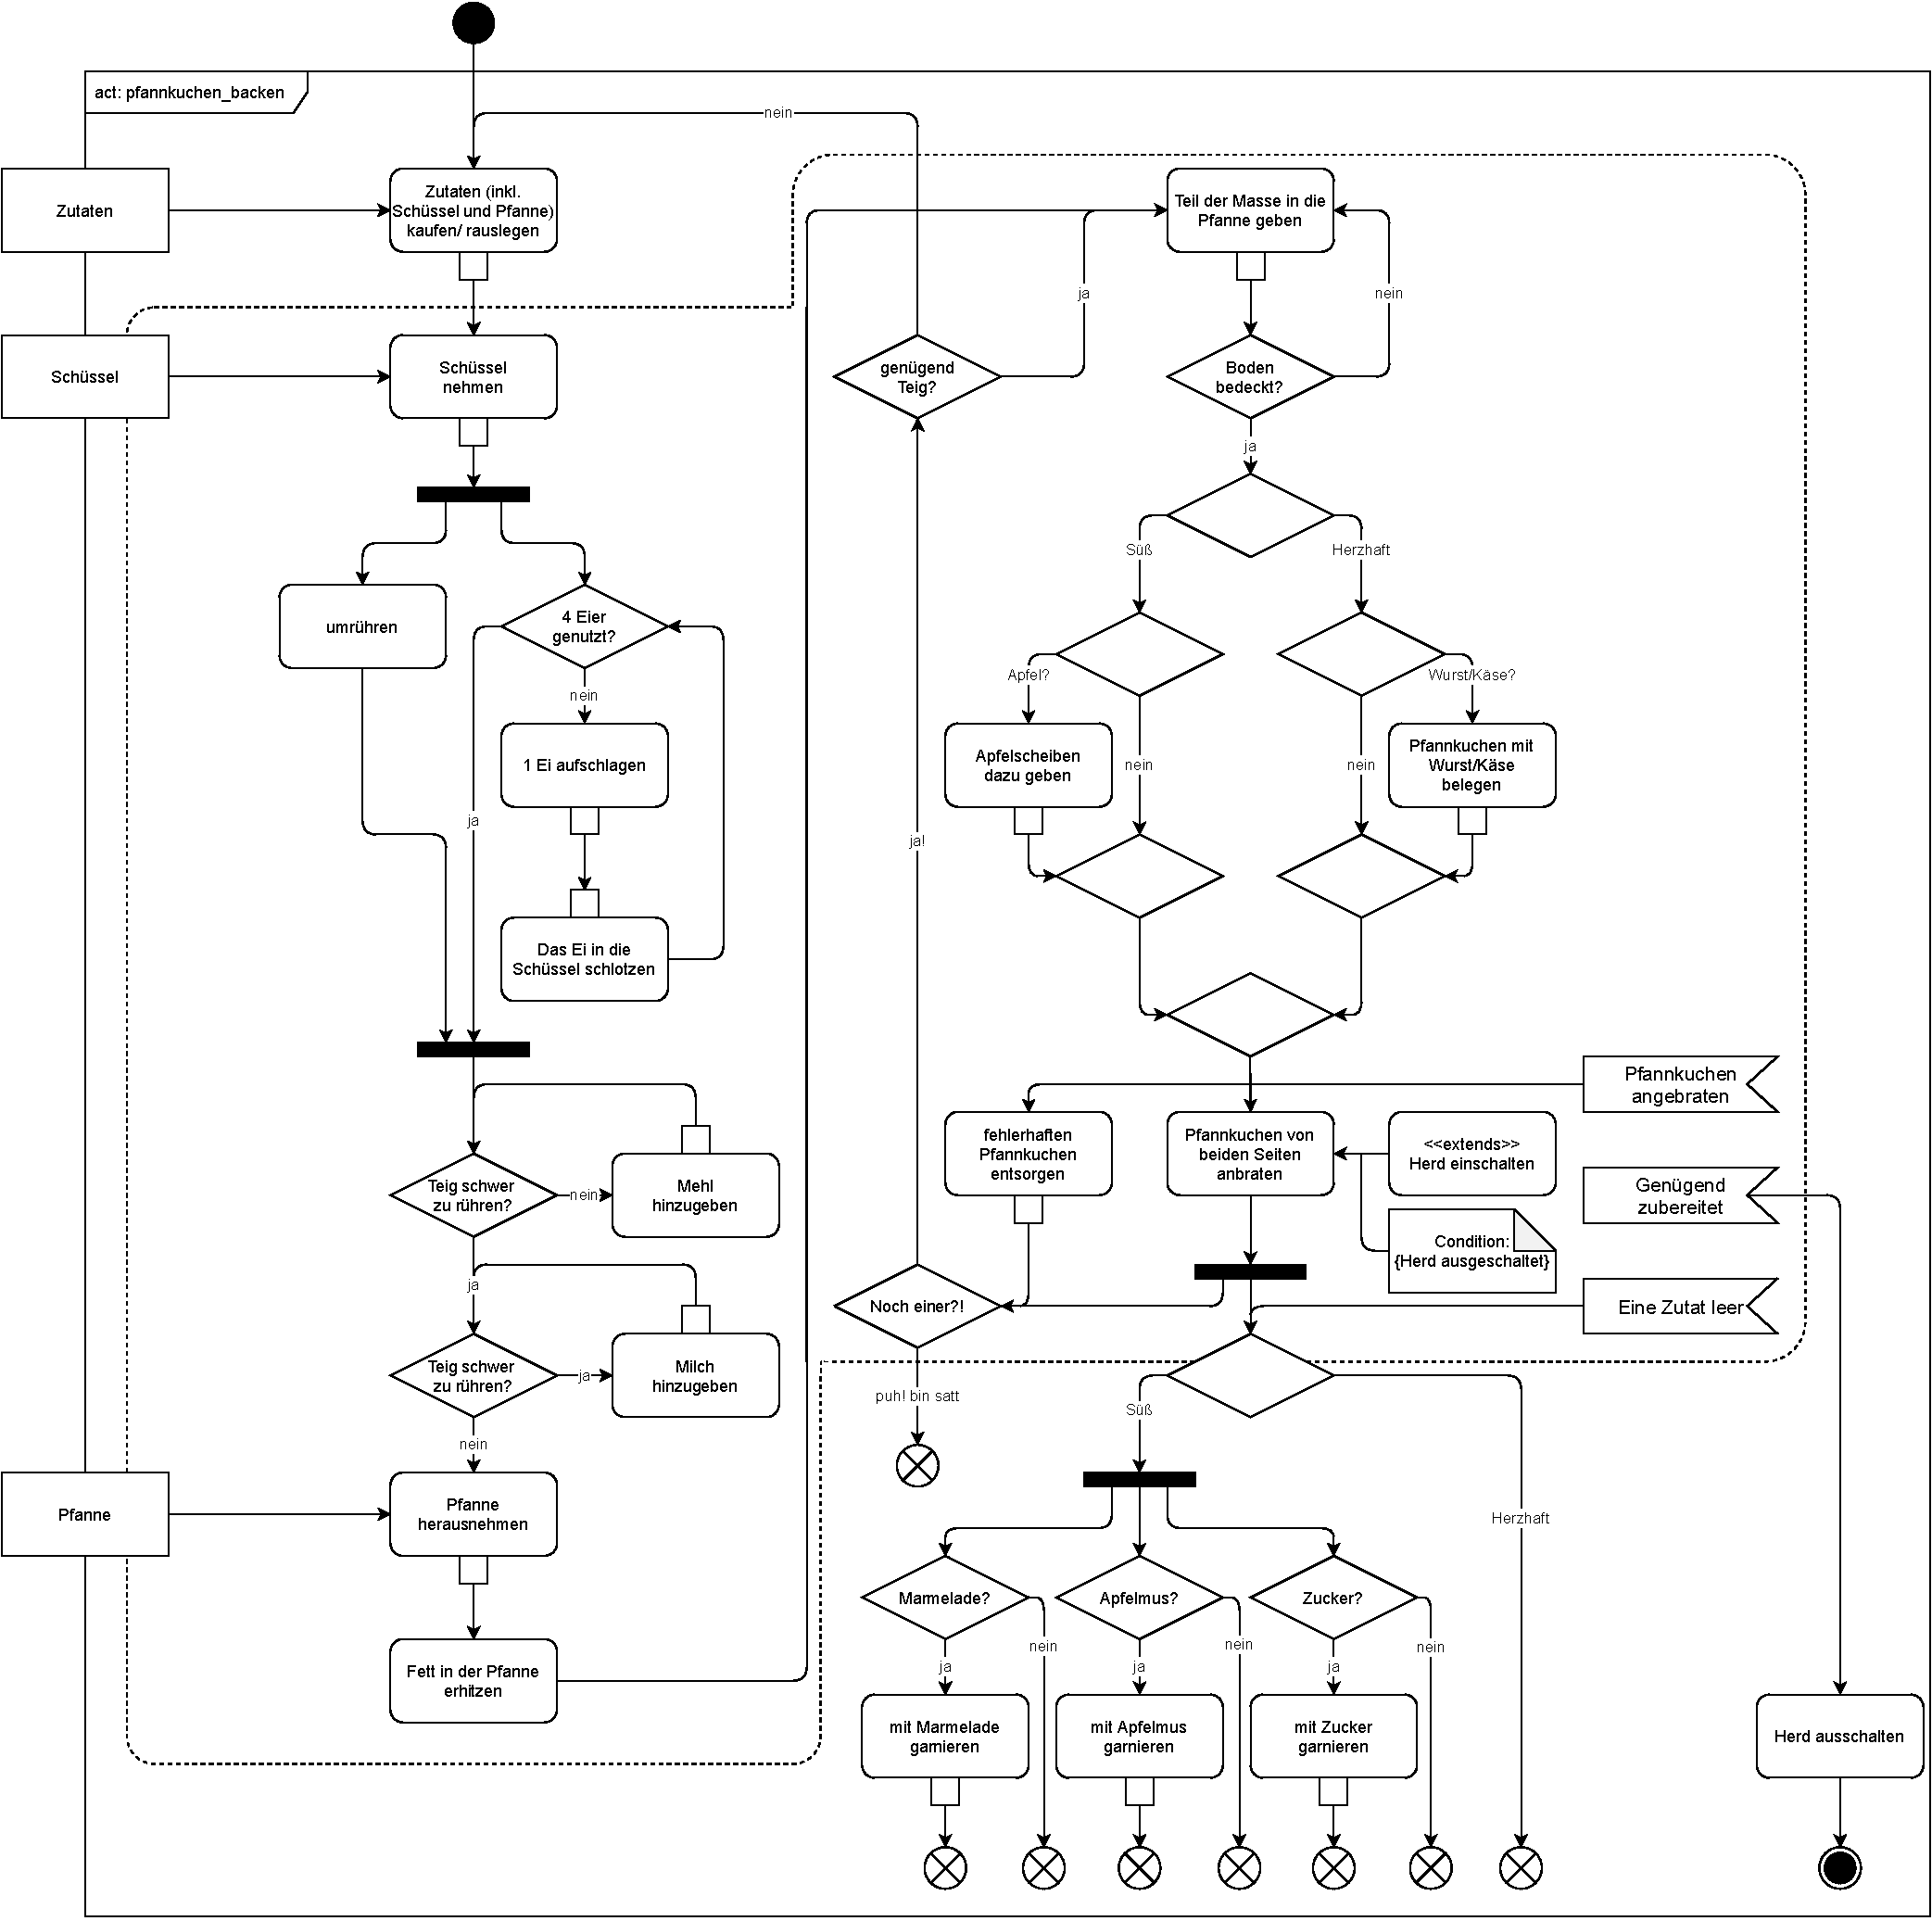
\includegraphics[width=\textwidth]{swt_wende_tim_h05_activity_diagram.pdf}
        \caption{\texttt{activity\_diagram}}
    \end{figure}

    \newpage
    Anmerkungen zum Diagramm:
    \begin{itemize}
        \item Jegliche Vor- und Nachbedingungen sind aus Komplexitätsgründen entfallen.
            Diese könnten durch wenige Veränderungen eingefügt werdem:
            \begin{itemize}
                \item Der Kauf der Zutaten kann parallel in einem festen, jedoch variablen Einkaufsladen stattfinden.
                \item Hierbei muss beachtet werden, ob eine Zutat bereits vorhanden ist
                \item Das Verspeisen der Pfannkuchen ist nach der Zubereitung möglich.
                    Dazu sollte man die Pfannkuchen jedoch vorher ein bisschen abkühlen lassen.
            \end{itemize} 
        \item Auf Grund verschiedener Quellen im Internet habe ich es mal gewagt \texttt{<<extends>>} zu nutzen.
            Sollte dies nicht erlaubt sein, könnte man den Herd einmalig am Anfang einschalten.
            Jedoch hat der jeweilige Nutzer, sollte er beim ersten Pfannkuchen bemerken, dass ihm Zutaten fehlen, den Herd umsonst eingeschaltet.
        \item Ich habe mal die Abfragen in die Rauten, anstatt an die Pfeile, daneben geschrieben.
            In neueren Versionen von UML ist dies erlaubt, sollte dies hier nicht der Fall sein, verzeihen Sie mir bitte diesen gestalterischen Fauxpas.
            Dies dient zur Verbesserung der Übersichtlichkeit.
        \item Zusätzlich habe ich das Diagramm in zwei Hälften aufgeteilt.
            Diese befinden sich natürlich ursprünglich untereinander, jedoch war mir hier das Format 1:20 zu unschön.
        \item Letztendlich habe ich mich dazu entschlossen alle Objekte als Objektknoten von außen zuzuführen.
            Diese werden einmalig initial an der jeweiligen Aktivität versendet, und am Ziel (hier nicht dargestellt: \gqq{pfannkuchen\_essen}) empfangen.
            Insgesamt handhabe ich das Diagramm eher wie ein Subflow, als wie eine eigenständige Aktivität.
            Die \gqq{Oberaktivität} könnte \texttt{pfannkuchen} sein, welche \texttt{zutaten\_kaufen}, \texttt{pfannkuchen\_backen} \& \texttt{pfannkuchen\_essen} enthält.
    \end{itemize}
\end{document}